\documentclass[theme=teal]{khmermath}
\usepackage{needspace}

\geometry{left=0.85cm, right=0.85cm, top=0.55cm, bottom=1.15cm, footskip=0.65cm}
\usepackage{colortbl}
\usepackage{tikz}
\usetikzlibrary{calc,shapes,arrows,intersections,through,backgrounds,shadows,decorations.pathmorphing,patterns}
\usepackage{fancyhdr}
\usepackage{multicol}
\usepackage{enumitem}

% -------------------------------------------------------------------------
% Korean Math Textbook Style Color Palette & Macros
% -------------------------------------------------------------------------
\definecolor{koreaTeal}{RGB}{0, 150, 155}       % Primary Header Teal/Cyan
\definecolor{koreaDarkTeal}{RGB}{0, 105, 110}   % Dark Teal Accent
\definecolor{koreaBeige}{RGB}{247, 244, 237}     % Concept Sidebar Beige (#F7F4EE)
\definecolor{koreaBeigeBorder}{RGB}{225, 218, 205}
\definecolor{koreaOrange}{RGB}{235, 115, 30}     % Problem Number Orange
\definecolor{koreaBlue}{RGB}{35, 110, 190}      % Standard Blue
\definecolor{koreaPurple}{RGB}{125, 50, 160}    % Purple Accent
\definecolor{koreaNumber}{RGB}{115, 125, 135}   % Problem Number Gray
\definecolor{koreaYellow}{RGB}{255, 246, 175}   % Yellow Highlight Tint

\definecolor{brandNavy}{RGB}{0, 105, 110}
\definecolor{brandBlue}{RGB}{0, 150, 155}
\definecolor{brandLightBlue}{RGB}{247, 244, 237}
\definecolor{brandCrimson}{RGB}{195, 35, 60}
\definecolor{brandCoral}{RGB}{235, 80, 75}
\definecolor{brandGold}{RGB}{215, 130, 10}
\definecolor{brandGoldBg}{RGB}{255, 252, 242}
\definecolor{brandTeal}{RGB}{0, 150, 155}
\definecolor{brandTealBg}{RGB}{244, 252, 250}
\definecolor{subtleGray}{RGB}{246, 251, 249}
\definecolor{cardBorder}{RGB}{220, 212, 198}

% Custom Header & Footer setup (Korean Textbook Style)
\pagestyle{fancy}
\fancyhf{}
\renewcommand{\headrulewidth}{0pt}
\renewcommand{\footrule}{\color{koreaTeal!60}\hrule height 0.6pt\vspace{3pt}}

\fancyfoot[L]{%
  \fontsize{8.5}{8.5}\selectfont\kml \color{koreaNumber}\textbf{\thepage}\ \vline\ \color{koreaDarkTeal}\textbf{៨. ប្រូបាប}%
}
\fancyfoot[C]{%
  \fontsize{8.5}{8.5}\selectfont\kby \color{koreaDarkTeal}\textbf{\ding{72}\ រៀបរៀងដោយ ៖ \textcolor{koreaDarkTeal}{ក្រូត រស្មី}\ \ding{72}}%
}
\fancyfoot[R]{%
  \fontsize{8.5}{8.5}\selectfont\kby \color{koreaDarkTeal}\textbf{ក្លឹបសិក្សាគណិតវិទ្យា PCM}\ \vline\ \color{koreaNumber}\textbf{\thepage}%
}

% Korean Header Banner
\newcommand{\koreanheader}[2]{%
  \noindent%
  \begin{tikzpicture}[x=1cm, y=1cm]
    \fill[koreaTeal, rounded corners=12pt] (0, 0.1) -- (0, 0.95) -- (3.8, 0.95) [rounded corners=0pt] -- (4.4, 0.1) -- cycle;
    \node[white, font=\fontsize{11}{11}\selectfont\kml\bfseries] at (1.9, 0.52) {#1};
    \node[anchor=west, font=\fontsize{18}{18}\selectfont\kml\bfseries, color=koreaDarkTeal] at (4.6, 0.42) {#2};
    \node[anchor=east, font=\fontsize{8.5}{8.5}\selectfont\kby, color=gray!80] at (19.2, 0.48) {$>$ ក្លឹបសិក្សាគណិតវិទ្យា PCM};
  \end{tikzpicture}%
  \vspace{3pt}%
}

% Yellow Formula Highlight Box
\newcommand{\koreahl}[1]{\colorbox{koreaYellow}{\fontsize{8.5}{8.5}\selectfont\textbf{#1}}}

% General Rule Box (Teal/Emerald Theme - ជាទូទៅ)
\newtcolorbox{khboxorange}[1][]{
  enhanced,
  colframe=brandNavy!40,
  colback=brandLightBlue,
  boxrule=0.7pt,
  arc=5.0pt,
  borderline west={3.5pt}{0pt}{brandNavy},
  drop fuzzy shadow=brandNavy!15,
  left=9pt, right=9pt, top=5.5pt, bottom=4.5pt,
  title={\fontsize{9.5}{9.5}\selectfont\kml\color{white}\ding{72}\ ជាទូទៅ},
  coltitle=white,
  colbacktitle=brandNavy,
  boxed title style={
    boxrule=0pt,
    arc=3.5pt,
    left=7pt, right=7pt, top=2.5pt, bottom=2.5pt
  },
  attach boxed title to top left={yshift*=-\tcboxedtitleheight/2, xshift=12pt},
  #1
}

% Feynman Intuition Box (Soft Light Emerald / Teal with bulb icon)
\newtcolorbox{khboxfeynman}[1][]{
  enhanced,
  colframe=koreaTeal!70,
  colback=brandTealBg,
  boxrule=0.7pt,
  arc=4.5pt,
  borderline west={3.5pt}{0pt}{koreaTeal},
  left=8pt, right=8pt, top=3.5pt, bottom=3pt,
  title={\fontsize{9}{9}\selectfont\kml\color{white}\ding{228}\ គន្លឹះយល់ដឹងបែប },
  coltitle=white,
  colbacktitle=koreaDarkTeal,
  boxed title style={
    boxrule=0pt,
    arc=3pt,
    left=6pt, right=6pt, top=2pt, bottom=2pt
  },
  attach boxed title to top left={yshift*=-\tcboxedtitleheight/2, xshift=10pt},
  #1
}

% Model Solution Box (Soft Beige / Blue)
\newtcolorbox{khboxsolution}[1][]{
  enhanced,
  colframe=brandBlue!60,
  colback=brandLightBlue,
  boxrule=0.65pt,
  arc=4pt,
  left=7pt, right=7pt, top=3.5pt, bottom=3pt,
  title={\fontsize{8.5}{8.5}\selectfont\kml\color{white}\ding{51}\ គំរូដំណោះស្រាយជាជំហានៗ (Model Solution)},
  coltitle=white,
  colbacktitle=brandBlue,
  boxed title style={
    boxrule=0pt,
    arc=2.5pt,
    left=5pt, right=5pt, top=1.8pt, bottom=1.8pt
  },
  attach boxed title to top left={yshift*=-\tcboxedtitleheight/2, xshift=8pt},
  #1
}

% Example / Card Item Box
\newtcolorbox{khcard}[1][]{
  enhanced,
  colframe=cardBorder,
  colback=white,
  boxrule=0.7pt,
  arc=3.5pt,
  left=6pt, right=6pt, top=2.8pt, bottom=2.8pt,
  #1
}

% Section Header Badge Macro
\newcommand{\khsection}[2]{%
  \Needspace*{3.5cm}%
  \vspace{3pt}%
  \noindent%
  \begin{tikzpicture}
    \fill[rounded corners=5pt, brandNavy!7] (0,0) rectangle (19.3, 0.70);
    \fill[rounded corners=4pt, brandNavy] (0.06, 0.06) rectangle (0.64, 0.64);
    \node[white, font=\fontsize{10}{10}\selectfont\bfseries] at (0.35, 0.35) {#1};
    \fill[brandGold, rounded corners=1pt] (0.74, 0.15) rectangle (0.78, 0.55);
    \node[anchor=west, font=\fontsize{11.5}{11.5}\selectfont\kml, color=brandCrimson] at (0.85, 0.35) {\textbf{#2}};
  \end{tikzpicture}%
  \vspace{2pt}%
}

% Korean Number Formatting for Exercises & Problems (01, 02, 03...)
\def\splitnum#1#2{%
  \color{koreaNumber!65}#1\color{koreaOrange}#2%
}
\newcommand{\koreannum}[1]{%
  \ifstrempty{#1}{}{%
    \mbox{%
      \fontsize{18}{18}\selectfont\bfseries%
      \ifnum#1<10\relax%
        \color{koreaNumber!65}0\color{koreaOrange}#1%
      \else%
        \expandafter\splitnum#1%
      \fi%
    }\,\ %
  }%
}

% Sub-question Badge (Crimson Rounded Square)
\newcommand{\khlabel}[1]{%
  \tikz[baseline=-0.6ex]{%
    \node[fill=brandCrimson, rounded corners=3.2pt, inner sep=2.2pt, minimum width=1.35em, minimum height=1.32em, text=white, font=\kml\fontsize{8}{8}\selectfont, align=center] (lbl) {\raisebox{0.2pt}{#1}};%
  }\,\ %
}

\newcommand{\exhead}[1]{\hangindent=24pt\hangafter=1\koreannum{#1}}

\setlength{\parindent}{0pt}
\setlength{\parskip}{2.5pt}
\setlength{\columnsep}{16pt}
\setlength{\columnseprule}{0.5pt}
\def\columnseprulecolor{\color{koreaTeal!40}}

\begin{document}

% =========================================================================
% PAGE 1: HEADER & SECTION 1 (PART 1)
% =========================================================================
\koreanheader{មេរៀនទី ៨}{ប្រូបាប}

\khsection{១}{ប្រូបាបនៃព្រឹត្តិការណ៍}

\begin{khboxfeynman}

  ប្រូបាប គឺគ្រាន់តែជាការវាស់វែងថា ៖ \textit{«តើលទ្ធផលដែលយើងចង់បាន មានឱកាសកើតឡើងប៉ុន្មាន ធៀបនឹងលទ្ធផលទាំងអស់ដែលអាចកើតមានឡើង ?»}
  \begin{equation*}
    P = \frac{\text{ចំនួនករណីដែលយើងចាប់អារម្មណ៍ (ករណីស្រប)}}{\text{ចំនួនលទ្ធផលទាំងអស់ដែលអាចកើតមាន (ករណីអាច)}}
  \end{equation*}
  \begin{itemize}[leftmargin=12pt, itemsep=1.5pt, topsep=1pt]
    \item[\color{brandCrimson}\ding{228}] បើព្រឹត្តិការណ៍មួយ\textbf{មិនអាចកើតឡើងសោះ} (មិនអាចទៅរួច) $\implies P = 0$ ($0\%$) ។
    \item[\color{brandNavy}\ding{228}] បើព្រឹត្តិការណ៍មួយ\textbf{ប្រាកដជាកើតឡើង $100\%$} (ព្រឹត្តិការណ៍ប្រាកដ) $\implies P = 1$ ($100\%$) ។
    \item[\color{koreaDarkTeal}\ding{228}] ដូចនេះ តម្លៃនៃប្រូបាបជានិច្ចកាលស្ថិតនៅក្នុងចន្លោះ ៖ \ \koreahl{$0 \le P \le 1$} ។
  \end{itemize}
\end{khboxfeynman}

\begin{khcard}
  \noindent\textbf{\color{koreaDarkTeal}\ding{70}\ ពិសោធន៍ ៖} បើគេចាប់យកអក្សរមួយចេញពីពាក្យ $\text{BANANA}$ តើលទ្ធផលដែលអាចកើតមានឡើងមានប៉ុន្មានរបៀប ?\\[2pt]
  \begin{minipage}[c]{0.68\linewidth}
    លទ្ធផលដែលអាចកើតមានឡើងគឺ $\{B, A, A, A, N, N\}$ ។
    \begin{itemize}[leftmargin=12pt, itemsep=1.5pt, topsep=1pt]
      \item[\color{brandCrimson}\ding{72}] លទ្ធផលដែលអាចកើតមានឡើងមាន $\{B, A, A, A, N, N\}$ ហៅថា \textbf{\color{brandCrimson}ព្រឹត្តិការណ៍អាច}($n = 6$) ។
      \item[\color{brandNavy}\ding{72}] បើគេប្រាថ្នាចាប់បានអក្សរ $A$ នោះការចាប់បានអក្សរ $A$ ហៅថា \textbf{\color{brandNavy}ព្រឹត្តិការណ៍ស្រប} ($m = 3$) ។
      \item[\color{koreaDarkTeal}\ding{228}] ផលធៀបរវាងចំនួនករណីស្របនឹងចំនួនករណីអាច ហៅថា \textbf{\color{koreaDarkTeal}ប្រូបាបនៃព្រឹត្តិការណ៍} មួយតាងដោយ $P$ ៖
      \[
        P = \frac{\text{ចំនួនករណីស្រប}}{\text{ចំនួនករណីអាច}} = \frac{3}{6} = \frac{1}{2} = 0.5 \ \text{ឬ}\ 50\% \text{ ។}
      \]
    \end{itemize}
  \end{minipage}\hfill
  \begin{minipage}[c]{0.25\linewidth}
    \centering
    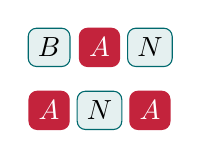
\begin{tikzpicture}[scale=0.8]
      \node[draw=brandNavy, fill=brandNavy!10, rounded corners=3pt, font=\bfseries, inner sep=3.5pt] at (0,0.6) {$B$};
      \node[draw=brandCrimson, fill=brandCrimson, text=white, rounded corners=3pt, font=\bfseries, inner sep=3.5pt] at (0.8,0.6) {$A$};
      \node[draw=brandNavy, fill=brandNavy!10, rounded corners=3pt, font=\bfseries, inner sep=3.5pt] at (1.6,0.6) {$N$};
      \node[draw=brandCrimson, fill=brandCrimson, text=white, rounded corners=3pt, font=\bfseries, inner sep=3.5pt] at (0,-0.4) {$A$};
      \node[draw=brandNavy, fill=brandNavy!10, rounded corners=3pt, font=\bfseries, inner sep=3.5pt] at (0.8,-0.4) {$N$};
      \node[draw=brandCrimson, fill=brandCrimson, text=white, rounded corners=3pt, font=\bfseries, inner sep=3.5pt] at (1.6,-0.4) {$A$};
    \end{tikzpicture}\\[2pt]
    {\fontsize{10}{7.5}\selectfont\color{brandCrimson}\textbf{អក្សរ $A$ មាន ៣ ក្នុងចំណោម ៦}}
  \end{minipage}
\end{khcard}

\begin{khboxorange}
  \textbf{ប្រូបាបនៃព្រឹត្តិការណ៍មួយកំណត់ដោយ ៖}
    \koreahl{$P = \frac{\text{ចំនួនករណីស្រប}}{\text{ចំនួនករណីអាច}}$}

\end{khboxorange}

\begin{khcard}
  \begin{minipage}[c]{0.70\linewidth}
    \exhead{1} គេសរសេរពាក្យ $\text{SUCCESSFUL}$ លើក្រដាសកាតុង រួចកាត់ជា $10$ សន្លឹក ហើយដាក់ក្នុងប្រអប់ ។ រកប្រូបាបដែលចាប់បាន ៖\\[1pt]
    \khlabel{ក} អក្សរ $U$ \hfill \khlabel{ខ} អក្សរ $S$ \hfill \khlabel{គ} អក្សរ $C$ \hfill \khlabel{ឃ} អក្សរ $S$ ឬ $U$
  \end{minipage}\hfill
  \begin{minipage}[c]{0.28\linewidth}
    \centering
    
\begin{tikzpicture}[scale=1]
      \foreach \x/\l/\c/\tc in {0/S/brandCrimson/white, 0.6/U/brandTeal/white, 1.2/C/brandNavy!15/brandNavy, 1.8/C/brandNavy!15/brandNavy, 2.4/E/brandNavy!15/brandNavy} {
        \node[draw=\c, fill=\c, text=\tc, rounded corners=1.5pt, font=\fontsize{10}{5.5}\selectfont\bfseries, inner sep=1.5pt] at (\x,0.38) {\l};
      }
      \foreach \x/\l/\c/\tc in {0/S/brandCrimson/white, 0.6/S/brandCrimson/white, 1.2/F/brandNavy!15/brandNavy, 1.8/U/brandTeal/white, 2.4/L/brandNavy!15/brandNavy} {
        \node[draw=\c, fill=\c, text=\tc, rounded corners=1.5pt, font=\fontsize{10}{5.5}\selectfont\bfseries, inner sep=1.5pt] at (\x,-0.30) {\l};
      }
    \end{tikzpicture}\\[1pt]
    {\fontsize{10}{6}\selectfont\color{brandCrimson}\textbf{សរុប ១០ អក្សរ ($S:3, U:2, C:2$)}}
  \end{minipage}
\end{khcard}


% =========================================================================
% PAGE 2: SECTION 1 CONT. (MODEL SOLUTION & PRACTICE PROBLEMS 02-07)
% =========================================================================

\begin{khboxsolution}
  \textbf{គំរូដំណោះស្រាយជា ៣ ជំហាន (សម្រាប់សិស្សយកជាគំរូ) ៖}
  \begin{itemize}[leftmargin=10pt, itemsep=1pt, topsep=1pt]
    \item \textbf{ជំហាន ១ ៖} $\text{SUCCESSFUL}$ មាន $10$ តួ $\implies$ \textbf{\color{brandCrimson}ចំនួនករណីអាចគឺ $10$} ។
    \item \textbf{ជំហាន ២ \& ៣ (ករណីស្រប និងគណនា $P$) ៖}
      \begin{itemize}[leftmargin=8pt, itemsep=1pt]
        \item \khlabel{ខ} អក្សរ $S$ មាន $3$ តួ $\implies$ \koreahl{$P(S) = \frac{3}{10} = 30\%$}
        \item \khlabel{គ} អក្សរ $C$ មាន $2$ តួ $\implies$ \koreahl{$P(C) = \frac{2}{10} = \frac{1}{5} = 20\%$}
        \item \khlabel{ឃ} អក្សរ $S$ ឬ $U$ មាន $3+2=5$ តួ $\implies$ \koreahl{$P(S \text{ ឬ } U) = \frac{5}{10} = \frac{1}{2} = 50\%$}
      \end{itemize}
  \end{itemize}
\end{khboxsolution}

\begin{khcard}
  \begin{minipage}[c]{0.70\linewidth}
    \exhead{2} បើគេជ្រើសរើសអក្សរមួយចេញពីពាក្យ $\text{PHNOMPENH}$ ដោយចៃដន្យ ៖\\[1pt]
    \khlabel{ក} រកចំនួនករណីអាច \hfill \khlabel{ខ} រក $P(H)$ និង $P(P)$\\
    \khlabel{គ} រកប្រូបាបដែលគេចាប់បានអក្សរ $P$ ឬ $N$
  \end{minipage}\hfill
  \begin{minipage}[c]{0.28\linewidth}
    \centering
    
\begin{tikzpicture}[scale=1]
      \foreach \x/\l/\c/\tc in {0/P/brandCrimson/white, 0.6/H/brandBlue/white, 1.2/N/brandTeal/white, 1.8/O/brandNavy!15/brandNavy, 2.4/M/brandNavy!15/brandNavy} {
        \node[draw=\c, fill=\c, text=\tc, rounded corners=1.5pt, font=\fontsize{10}{5.5}\selectfont\bfseries, inner sep=1.5pt] at (\x,0.38) {\l};
      }
      \foreach \x/\l/\c/\tc in {0/P/brandCrimson/white, 0.6/E/brandNavy!15/brandNavy, 1.2/N/brandTeal/white, 1.8/H/brandBlue/white} {
        \node[draw=\c, fill=\c, text=\tc, rounded corners=1.5pt, font=\fontsize{10}{5.5}\selectfont\bfseries, inner sep=1.5pt] at (\x+0.3,-0.30) {\l};
      }
    \end{tikzpicture}\\[1pt]
    {\fontsize{6}{6}\selectfont\color{brandNavy}\textbf{សរុប ៩ អក្សរ}}
  \end{minipage}
\end{khcard}

\begin{khcard}
  \begin{minipage}[c]{0.76\linewidth}
    \exhead{3} ក្នុងថង់មានឃ្លីស $5$ ខ្មៅ $12$ និងខៀវ $8$ គ្រាប់ ។ រតនៈលូកយកឃ្លីមួយដោយចៃដន្យ ៖\\[1pt]
    \khlabel{ក} រកប្រូបាបដែលចាប់បានឃ្លីពណ៌ស \hfill
    \khlabel{ខ} រកប្រូបាបចាប់បានឃ្លីពណ៌ខ្មៅ ឬពណ៌ខៀវ
  \end{minipage}\hfill
  \begin{minipage}[c]{0.22\linewidth}
    \centering
    \begin{tikzpicture}[scale=2]
      \draw[thick, color=brandNavy, fill=brandTealBg, rounded corners=5pt] (-0.85,-0.55) rectangle (0.85,0.55);
      \fill[white, draw=gray, thick] (-0.45,-0.2) circle (0.17) node[font=\fontsize{4.5}{4.5}\selectfont\bfseries, text=black] {ស:5};
      \fill[black] (0.4,-0.2) circle (0.17) node[font=\fontsize{4.5}{4.5}\selectfont\bfseries, text=white] {ខ្មៅ:12};
      \fill[brandBlue] (0,0.22) circle (0.17) node[font=\fontsize{4.5}{4.5}\selectfont\bfseries, text=white] {ខៀវ:8};
      \node[below, font=\fontsize{10}{5.5}\selectfont\kml, color=brandNavy] at (0,-0.58) {សរុប $25$ គ្រាប់};
    \end{tikzpicture}
  \end{minipage}
\end{khcard}

\begin{khcard}
  \begin{minipage}[c]{0.76\linewidth}
    \exhead{4} ថង់មួយមានឃ្លីបួនដែលបង់អក្សរ $a, A, b, B$ ។ ពិសិដ្ឋចាប់យកឃ្លីម្ដងពីរចេញពីថង់ ។ ចូររៀបរាប់ព្រឹត្តិការណ៍អាច រួចគណនាប្រូបាបដែលចាប់បានឃ្លីពីរមានអក្សរតូចមួយនិងធំមួយ ។
  \end{minipage}\hfill
  \begin{minipage}[c]{0.22\linewidth}
    \centering
    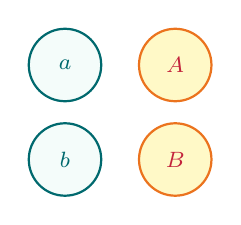
\begin{tikzpicture}[scale=2]
      \fill[brandTealBg, draw=brandNavy, thick] (-0.35,0.3) circle (0.23) node[font=\bfseries\footnotesize, color=brandNavy] {$a$};
      \fill[koreaYellow!70, draw=koreaOrange, thick] (0.35,0.3) circle (0.23) node[font=\bfseries\footnotesize, color=brandCrimson] {$A$};
      \fill[brandTealBg, draw=brandNavy, thick] (-0.35,-0.3) circle (0.23) node[font=\bfseries\footnotesize, color=brandNavy] {$b$};
      \fill[koreaYellow!70, draw=koreaOrange, thick] (0.35,-0.3) circle (0.23) node[font=\bfseries\footnotesize, color=brandCrimson] {$B$};
    \end{tikzpicture}
  \end{minipage}
\end{khcard}

\begin{khcard}
  \begin{minipage}[c]{0.76\linewidth}
    \exhead{5} គេធ្វើតេស្តលើអំពូលភ្លើង $500$ គ្រឿង រកឃើញមានអំពូល $4$ ខូច ៖\\[1pt]
    \khlabel{ក} រកប្រូបាបនៃការរកឃើញអំពូលភ្លើងខូចនេះ\\
    \khlabel{ខ} បើត្រូវលក់ $8500$ គ្រឿង តើត្រូវត្រៀមអំពូលប៉ុន្មានដើម្បីថែមឱ្យអតិថិជន ?
  \end{minipage}\hfill
  \begin{minipage}[c]{0.22\linewidth}
    \centering
    \begin{tikzpicture}[scale=2]
      \draw[thick, fill=koreaYellow!85] (0,0.25) circle (0.26);
      \node[above, font=\fontsize{9}{5}\selectfont\bfseries, color=brandNavy] at (0,0.52) {ល្អ: 496};
      \draw[thick, fill=gray!20] (0.9,0.25) circle (0.26);
      \draw[very thick, color=brandCrimson] (0.7,0.05) -- (1.1,0.45);
      \draw[very thick, color=brandCrimson] (0.7,0.45) -- (1.1,0.05);
      \node[above, font=\fontsize{9}{5}\selectfont\bfseries, color=brandCrimson] at (0.9,0.52) {ខូច: 4};
    \end{tikzpicture}
  \end{minipage}
\end{khcard}

\begin{khcard}
  \exhead{6} ថង់មួយមានឃ្លីស និងខ្មៅសរុប $15$ គ្រាប់ ។ គេចាប់យកម្ដងមួយហើយដាក់ចូលវិញ រហូតដល់គ្រប់ $100$ ដង ដោយឃើញឃ្លីខ្មៅចេញ $40$ ដង ។ ចូររកចំនួនឃ្លីខ្មៅ និងពណ៌ស ។
\end{khcard}

\begin{khcard}
  \begin{minipage}[c]{0.76\linewidth}
    \exhead{7} ថង់មួយមានឃ្លីខ្មៅ $4$ និងស $2$ ៖\\[1pt]
    \khlabel{ក} បើ ក ចាប់យក $1$ រកប្រូបាបដែល ក ចាប់បានឃ្លីខ្មៅ\\
    \khlabel{ខ} ឧបមា ក ចាប់បានខ្មៅ (មិនដាក់វិញ) រួច ខ ចាប់បន្ត ។ រកប្រូបាបដែល ខ ចាប់បានខ្មៅ
  \end{minipage}\hfill
  \begin{minipage}[c]{0.22\linewidth}
    \centering
    \begin{tikzpicture}[scale=2]
      \draw[thick, color=brandNavy, fill=brandTealBg, rounded corners=5pt] (-0.75,-0.48) rectangle (0.75,0.48);
      \fill[black] (-0.35,0.18) circle (0.14);
      \fill[black] (0.35,0.18) circle (0.14);
      \fill[black] (-0.35,-0.2) circle (0.14);
      \fill[black] (0.35,-0.2) circle (0.14);
      \fill[white, draw=gray, thick] (0,0.18) circle (0.14);
      \fill[white, draw=gray, thick] (0,-0.2) circle (0.14);
      \node[below, font=\fontsize{10}{5}\selectfont\kml, color=brandNavy] at (0,-0.50) {ខ្មៅ 4 , ស 2};
    \end{tikzpicture}
  \end{minipage}
\end{khcard}

 %=========================================================================
% PAGE 3: SECTION 2 (COMPLEMENTARY EVENTS WITH FEYNMAN & MODEL SOLUTION)
% =========================================================================
\khsection{២}{ប្រូបាបនៃព្រឹត្តិការណ៍បំពេញ}

\begin{khboxfeynman}
  \textbf{ហេតុអ្វីបានជា $P + P' = 1$ ? (ការយល់ដឹងបែប Feynman)}\\[1.5pt]
  គិតដូចនំពេញមួយ ($100\% = 1$) ៖ រឿងមួយ បើវាមិនកើតឡើងទេ វាច្បាស់ជាមិនកើត គ្មានជម្រើសទីបីឡើយ!
  \begin{center}
    \begin{tikzpicture}[scale=1]
      \fill[brandTeal, rounded corners=3pt] (0,0) rectangle (3.2, 0.48);
      \node[white, font=\fontsize{8}{8}\selectfont\bfseries] at (1.6, 0.24) {ភ្លៀង $P = 30\%$};
      \fill[koreaOrange!85, rounded corners=3pt] (3.28,0) rectangle (10, 0.48);
      \node[white, font=\fontsize{8}{8}\selectfont\bfseries] at (6.64, 0.24) {មិនភ្លៀង $P' = 70\%$};
      \draw[thick, color=brandNavy, decorate, decoration={brace, amplitude=4pt, mirror}] (0,-0.08) -- (10,-0.08) node[midway, below=4pt, font=\fontsize{8}{8}\selectfont\kml, color=brandNavy] {ផលបូកប្រូបាបជានិច្ចកាលស្មើ $1$ ($100\%$) ៖ $P + P' = 1$};
    \end{tikzpicture}
  \end{center}
  \begin{itemize}[leftmargin=12pt, itemsep=1.5pt, topsep=1pt]
    \item \textbf{គន្លឹះដោះស្រាយ ៖} នៅពេលលំហាត់សួររកប្រូបាបដែលស្មុគស្មាញ (ដូចជាពាក្យ «យ៉ាងតិចមួយ») វិធីដែលលឿន និងឆ្លាតបំផុតគឺគណនាតាមព្រឹត្តិការណ៍បំពេញ ៖ \ \koreahl{$P' = 1 - P$} ។
  \end{itemize}
\end{khboxfeynman}

\begin{khboxorange}
  \textbf{បើ $P'$ ជាប្រូបាបបំពេញនៃ $P$ នោះ ៖}
  \begin{equation*}
    \koreahl{$P + P' = 1 \iff P' = 1 - P$}
  \end{equation*}
\end{khboxorange}

\begin{khcard}
  \begin{minipage}[c]{0.76\linewidth}
    \exhead{1} ថង់មួយមានឃ្លីពណ៌ស $4$ គ្រាប់ និងពណ៌ខ្មៅ $5$ គ្រាប់ ។ សុភារិទ្ធបានលូកចាប់ឃ្លីមួយពីថង់ ។\\[2pt]
    \khlabel{ក} រកប្រូបាបដែលចាប់បានឃ្លីពណ៌ស ។\hfill
    \khlabel{ខ} រកប្រូបាបដែលចាប់បានឃ្លីពណ៌ខ្មៅ ។
  \end{minipage}\hfill
  \begin{minipage}[c]{0.22\linewidth}
    \centering
    \begin{tikzpicture}[scale=1.5]
      \draw[thick, color=brandNavy, fill=brandTealBg, rounded corners=6pt] (-0.8,-0.65) rectangle (0.8,0.65);
      \fill[white, draw=gray, thick] (-0.35,-0.15) circle (0.22) node[font=\fontsize{5.5}{5.5}\selectfont\bfseries, text=black] {ស:4};
      \fill[black] (0.35,-0.15) circle (0.22) node[font=\fontsize{5.5}{5.5}\selectfont\bfseries, text=white] {ខ្មៅ:5};
      \node[below, font=\fontsize{10}{6.5}\selectfont\kml, color=brandNavy] at (0,-0.7) {សរុប $9$ គ្រាប់};
    \end{tikzpicture}
  \end{minipage}
\end{khcard}

\begin{khcard}
  \begin{minipage}[c]{0.78\linewidth}
    \exhead{2} គេបោះកាក់ម្ដងពីរ ។ ចូររកប្រូបាបដែលបោះបានអក្សរពីរផ្សេងគ្នា រួចទាញរកប្រូបាបដែលបោះបានអក្សរពីរដូចគ្នា ។
  \end{minipage}\hfill
  \begin{minipage}[c]{0.20\linewidth}
    \centering
    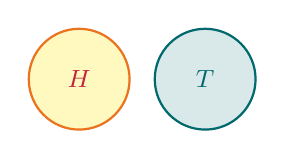
\begin{tikzpicture}[scale=2]
      \fill[koreaYellow!80, draw=koreaOrange, thick] (-0.4,0) circle (0.32) node[font=\bfseries\small, color=brandCrimson] {$H$};
      \fill[brandNavy!15, draw=brandNavy, thick] (0.4,0) circle (0.32) node[font=\bfseries\small, color=brandNavy] {$T$};
    \end{tikzpicture}
  \end{minipage}
\end{khcard}

\begin{khboxsolution}
  \textbf{គំរូដំណោះស្រាយតាមព្រឹត្តិការណ៍បំពេញ ៖}
  \begin{itemize}[leftmargin=12pt, itemsep=2pt, topsep=1pt]
    \item លទ្ធផលអាចបោះកាក់ ២ ដង គឺ ៖ $S = \{HH, HT, TH, TT\} \implies$ ចំនួនករណីអាចគឺ $4$ ។
    \item ព្រឹត្តិការណ៍បោះបាន «អក្សរពីរផ្សេងគ្នា» គឺ $\{HT, TH\} \implies 2$ ករណីស្រប ៖
      \[ P(\text{ផ្សេងគ្នា}) = \frac{2}{4} = \frac{1}{2} \]
    \item \textbf{ទាញរក «អក្សរពីរដូចគ្នា» (ព្រឹត្តិការណ៍បំពេញ) ៖} ដោយសារព្រឹត្តិការណ៍ «ដូចគ្នា» ជាព្រឹត្តិការណ៍បំពេញនៃ «ផ្សេងគ្នា» យើងមិនចាំបាច់រាប់សាឡើងវិញឡើយ ៖
      \[ P(\text{ដូចគ្នា}) = 1 - P(\text{ផ្សេងគ្នា}) = 1 - \frac{1}{2} = \koreahl{$\frac{1}{2}$} \]
  \end{itemize}
\end{khboxsolution}

\begin{khcard}
  \exhead{3} ថង់មួយមានឃ្លីបួនដែលបង់អក្សរ $a, A, b, B$ ។ គេបានចាប់យកឃ្លីម្ដងពីរចេញពីថង់ ។ គណនាប្រូបាបដែលចាប់បានឃ្លីពីរដែលមានអក្សរធំទាំងពីរ រួចទាញរកប្រូបាបដែលចាប់បានអក្សរតូចមួយយ៉ាងតិច ។
\end{khcard}

\begin{khcard}
  \begin{minipage}[c]{0.78\linewidth}
    \exhead{4} ក្នុងថង់មួយដែលមានតែឃ្លីពណ៌ស និងពណ៌ខ្មៅ ។ ចូររកប្រូបាបដែលចាប់បានឃ្លីពណ៌ស ដោយដឹងថាប្រូបាបដែលចាប់បានឃ្លីពណ៌ខ្មៅស្មើនឹង $\frac{2}{5}$ ។
  \end{minipage}\hfill
  \begin{minipage}[c]{0.20\linewidth}
    \centering
    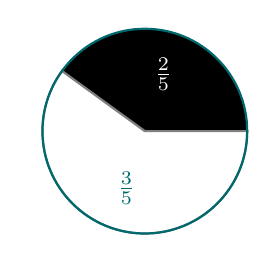
\begin{tikzpicture}[scale=2]
      \fill[black] (0,0) -- (0:0.65) arc (0:144:0.65) -- cycle;
      \fill[white, draw=gray, thick] (0,0) -- (144:0.65) arc (144:360:0.65) -- cycle;
      \draw[thick, color=brandNavy] (0,0) circle (0.65);
      \node[font=\bfseries, text=white] at (72:0.38) {$\frac{2}{5}$};
      \node[font=\bfseries, text=brandNavy] at (252:0.38) {$\frac{3}{5}$};
    \end{tikzpicture}
  \end{minipage}
\end{khcard}

\begin{khcard}
  \begin{minipage}[c]{0.74\linewidth}
    \exhead{5} ក្រុមហ៊ុនមួយមានបុគ្គលិកចំនួន $250$ នាក់ ។ គេដឹងថាអ្នកដែលធ្វើដំណើរដោយរថយន្តផ្ទាល់ខ្លួនមានចំនួន $50$ នាក់ ។ រកប្រូបាបដែលធ្វើដំណើរដោយមធ្យោបាយដទៃទៀត ។
  \end{minipage}\hfill
  \begin{minipage}[c]{0.24\linewidth}
    \centering
    \begin{tikzpicture}[scale=1.5]
      \fill[brandCrimson, rounded corners=2pt] (0,0) rectangle (0.65,0.4);
      \node[white, font=\bfseries] at (0.32,0.2) {50};
      \fill[brandNavy!20, rounded corners=2pt] (0.72,0) rectangle (2.5,0.4);
      \node[brandNavy, font=\bfseries] at (1.61,0.2) {ដទៃ: 200};
      \node[below, font=\fontsize{10}{5.5}\selectfont\kml, color=brandNavy] at (1.25,-0.05) {សរុប 250 នាក់};
    \end{tikzpicture}
  \end{minipage}
\end{khcard}


% =========================================================================
% PAGE 4: SECTION 3 (MULTI-STAGE EXPERIMENTS WITH GRID TABLE & TREE DIAGRAM)
% =========================================================================
\khsection{៣}{ប្រូបាបនៃព្រឹត្តិការណ៍ដែលពិសោធន៍ច្រើនដង}

\begin{khboxfeynman}
  \textbf{គន្លឹះដោះស្រាយការពិសោធន៍ច្រើនដង ៖}\\[1pt]
  \begin{minipage}[c]{0.64\linewidth}
    \textbf{១. ដ្យាក្រាមដើមឈើ ៖} សម្រាប់កាក់ ២-៣ ដង និងលំដាប់កូន ($B/G$) ។\\
    \textbf{២. តារាងក្រឡា ($36$ ករណី) ៖} ស័ក្តិសមបំផុតសម្រាប់គ្រាប់ឡុកឡាក់ ២ ដង ។
  \end{minipage}\hfill
  \begin{minipage}[c]{0.34\linewidth}
    \centering
    \begin{tikzpicture}[scale=2, level distance=0.70cm, sibling distance=1.05cm,
      edge from parent/.style={draw=brandNavy, line width=0.45pt},
      every node/.style={font=\fontsize{9}{5}\selectfont\bfseries}]
      \node[circle, draw=brandNavy, fill=brandTealBg, inner sep=0.9pt] {កាក់}
        child { node[circle, draw=brandCrimson, fill=koreaYellow!80, inner sep=0.9pt] {$H$}
          child { node[fill=brandLightBlue, draw=brandNavy, inner sep=0.6pt] {$HH$} }
          child { node[fill=brandLightBlue, draw=brandNavy, inner sep=0.6pt] {$HT$} }
        }
        child { node[circle, draw=brandNavy, fill=brandNavy!15, inner sep=0.9pt] {$T$}
          child { node[fill=brandLightBlue, draw=brandNavy, inner sep=0.6pt] {$TH$} }
          child { node[fill=brandLightBlue, draw=brandNavy, inner sep=0.6pt] {$TT$} }
        };
    \end{tikzpicture}
  \end{minipage}
\end{khboxfeynman}

\begin{khcard}
  \exhead{1} ចូរអ្នករក ករណីអាចបោះកាក់ ៖ \ \khlabel{ក} ១ ដង \ \khlabel{ខ} ២ ដង \ \khlabel{គ} ៣ ដង 
\end{khcard}
\begin{khcard}
	\exhead{2} ចូរអុ្នករកករណីអាចបោះឡុកឡាក់ ៖ \ \khlabel{ក} ១ ដង \ \khlabel{ខ} ២ ដង
\end{khcard}

\begin{khcard}
  \exhead{3} គេបោះកាក់មួយ ២ ដង ៖ \ \khlabel{ក} $P(TT)$ \ \khlabel{ខ} $P(HH)$ \ \khlabel{គ} $P(\ge 1H)$ \ \khlabel{ឃ} $P(\ge 1T)$
\end{khcard}
\begin{khcard}

	\exhead{4} គេបោះកាក់មួយ ៣ ដង ៖ \ \khlabel{ក} $P(TTT)$ \ \khlabel{ខ} $P(\le 1H)$ \ \khlabel{គ} $P(\ge 1H)$ \ \khlabel{ឃ} $P(\ge 2T)$
\end{khcard}

\begin{khcard}
  \exhead{5} គ្រាប់ឡុកឡាក់មួយត្រូវបានគេបោះវាចំនួនពីរដង ៖\\[1pt]
  \khlabel{ក} សរសេរព្រឹត្តិការណ៍អាចទាំងអស់ \hfill
  \khlabel{ខ} រក $P(\text{បូក } 5)$ \hfill
  \khlabel{គ} រក $P(\text{បូក } 9)$\\
  \khlabel{ឃ} រកប្រូបាបដែលផលបូកលេខ $\ge 8$ \hfill
  \khlabel{ង} រកប្រូបាបដែលផលបូកលេខជាការេប្រាកដ
\end{khcard}

\begin{khboxsolution}
  \noindent\textbf{តារាងផលបូកគ្រាប់ឡុកឡាក់ ២ ដង ($6 \times 6 = 36$ ករណីអាច) ៖}\\[1pt]
  \begin{minipage}[c]{0.50\linewidth}
    \centering
    \fontsize{9}{7.5}\selectfont
    \renewcommand{\arraystretch}{0.94}
    \setlength{\tabcolsep}{2.8pt}
    \begin{tabular}{|c|c|c|c|c|c|c|}
      \hline
      \rowcolor{brandNavy!15} \textbf{+} & \textbf{1} & \textbf{2} & \textbf{3} & \textbf{4} & \textbf{5} & \textbf{6} \\
      \hline
      \textbf{1} & 2 & 3 & 4 & \cellcolor{koreaYellow!80}\textbf{5} & 6 & 7 \\
      \hline
      \textbf{2} & 3 & 4 & \cellcolor{koreaYellow!80}\textbf{5} & 6 & 7 & 8 \\
      \hline
      \textbf{3} & 4 & \cellcolor{koreaYellow!80}\textbf{5} & 6 & 7 & 8 & \cellcolor{koreaOrange!40}\textbf{9} \\
      \hline
      \textbf{4} & \cellcolor{koreaYellow!80}\textbf{5} & 6 & 7 & 8 & \cellcolor{koreaOrange!40}\textbf{9} & 10 \\
      \hline
      \textbf{5} & 6 & 7 & 8 & \cellcolor{koreaOrange!40}\textbf{9} & 10 & 11 \\
      \hline
      \textbf{6} & 7 & 8 & \cellcolor{koreaOrange!40}\textbf{9} & 10 & 11 & 12 \\
      \hline
    \end{tabular}
  \end{minipage}\hfill
  \begin{minipage}[c]{0.48\linewidth}
    \fontsize{7.0}{8.2}\selectfont
    \begin{itemize}[leftmargin=6pt, itemsep=1.0pt, topsep=0pt]
      \item \textbf{បូក $5$ ៖} \koreahl{$P = \frac{4}{36} = \frac{1}{9}$}
      \item \textbf{បូក $9$ ៖} \koreahl{$P = \frac{4}{36} = \frac{1}{9}$}
      \item \textbf{បូក $\ge 8$ ៖} \koreahl{$P = \frac{15}{36} = \frac{5}{12}$}
      \item \textbf{ជាការេ ($4, 9$) ៖} \koreahl{$P = \frac{3+4}{36} = \frac{7}{36}$}
    \end{itemize}
  \end{minipage}
\end{khboxsolution}

\begin{khcard}
  \exhead{6} បោះគ្រាប់ឡុកឡាក់ ២ ដង ។ រកប្រូបាបដែលបោះបានលេខដូចគ្នា\penalty10000\ ?
\end{khcard}

\begin{khcard}
  \begin{minipage}[c]{0.74\linewidth}
    \exhead{7} គ្រួសារមួយចង់បានបុត្រតាមលំដាប់ $BGB$ ($B$: ប្រុស, $G$: ស្រី) ។ រកប្រូបាបជាភាគរយ\penalty10000\ ?\\[1.5pt]
  \end{minipage}\hfill
  \begin{minipage}[c]{0.24\linewidth}
    \centering
    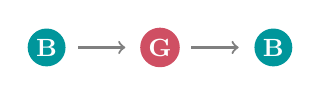
\begin{tikzpicture}[scale=2]
      \node[circle, fill=brandBlue, text=white, font=\fontsize{9}{5.5}\selectfont\bfseries, inner sep=1.4pt] at (0,0) {B};
      \draw[->, thick, color=gray] (0.20,0) -- (0.50,0);
      \node[circle, fill=brandCrimson!80, text=white, font=\fontsize{9}{5.5}\selectfont\bfseries, inner sep=1.4pt] at (0.72,0) {G};
      \draw[->, thick, color=gray] (0.92,0) -- (1.22,0);
      \node[circle, fill=brandBlue, text=white, font=\fontsize{9}{5.5}\selectfont\bfseries, inner sep=1.4pt] at (1.44,0) {B};
    \end{tikzpicture}\\[1pt]
    {\fontsize{9}{5.5}\selectfont\color{brandNavy}\textbf{លំដាប់ $BGB$}}
  \end{minipage}
\end{khcard}
\begin{khcard}
	 \exhead{8} បោះឡុកឡាក់មួយចំនួន ២ ដង ចូររកប្រូបាប៖ \ \khlabel{ក} លេខដូចគ្នា \ \khlabel{ខ} ផលបូកស្មើ $10$
\end{khcard}


% =========================================================================
% PAGE 5: SECTION 4 (PRACTICE EXERCISES 1 TO 8)
% =========================================================================
\khsection{៤}{លំហាត់អនុវត្តន៍បន្ថែម}

\begin{multicols}{2}
  \noindent
  % PROBLEM 1
  \begin{minipage}{\linewidth}
    \exhead{1} គេចាប់យកអក្សរមួយនៃពាក្យ $\text{PHNOMPENH}$ ដោយចៃដន្យ ។ ចូររកប្រូបាបដែលចាប់បាន ៖\\[1.5pt]
    \khlabel{ក} អក្សរ $P$ \hfill \khlabel{ខ} អក្សរ $H$\\
    \khlabel{គ} អក្សរ $O$ ឬ $M$ \hfill \khlabel{ឃ} អក្សរ $P$ ឬ $N$
  \end{minipage}

  \vspace{6pt}
  % PROBLEM 2 (Side-by-side)
  \begin{minipage}{\linewidth}
    \begin{minipage}[c]{0.56\linewidth}
      \exhead{2} ចូររកប្រូបាបនៃគ្រាប់ឡុកឡាក់ដែលចេញលេខ $1$ ដល់លេខ $4$ ។
    \end{minipage}\hfill
    \begin{minipage}[c]{0.42\linewidth}
      \centering
      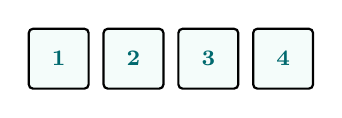
\begin{tikzpicture}[scale=1]
        \foreach \x/\n in {0/1, 0.95/2, 1.9/3, 2.85/4} {
          \draw[thick, fill=brandTealBg, rounded corners=1.5pt] (\x,0) rectangle (\x+0.76,0.76);
          \node[font=\bfseries\footnotesize, color=brandNavy] at (\x+0.38,0.38) {\n};
        }
      \end{tikzpicture}
    \end{minipage}
  \end{minipage}

  \vspace{6pt}
  % PROBLEM 3 (Side-by-side)
  \begin{minipage}{\linewidth}
    \begin{minipage}[c]{0.68\linewidth}
      \exhead{3} ក្នុងវិញ្ញាសាគប់ព្រួញមួយ តើប្រូបាបដែលគប់លើផ្ទៃឆ្នូតស្មើនឹងផ្ទៃមិនឆ្នូត ឬទេ\penalty10000\ ?
    \end{minipage}\hfill
    \begin{minipage}[c]{0.30\linewidth}
      \centering
      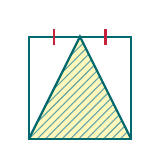
\begin{tikzpicture}[scale=1]
        \coordinate (A) at (0,1.3);
        \coordinate (B) at (1.3,1.3);
        \coordinate (C) at (1.3,0);
        \coordinate (D) at (0,0);
        \coordinate (M) at (0.65,1.3);
        \fill[koreaYellow!85] (D) -- (M) -- (C) -- cycle;
        \draw[pattern=north east lines, pattern color=brandNavy!60] (D) -- (M) -- (C) -- cycle;
        \draw[thick, color=brandNavy] (A) rectangle (C);
        \draw[thick, color=brandNavy] (D) -- (M) -- (C);
        \draw[thick, color=brandCrimson] (0.325, 1.2) -- (0.325, 1.4);
        \draw[thick, color=brandCrimson] (0.975, 1.2) -- (0.975, 1.4);
      \end{tikzpicture}
    \end{minipage}
  \end{minipage}

  \vspace{6pt}
  % PROBLEM 4
  \begin{minipage}{\linewidth}
    \exhead{4} ខាងក្រោមនេះជាព្រឹត្តិការណ៍អាចនៃការបោះកាក់ $4$ ដង ៖\\[1pt]
    \begin{center}
      \fontsize{6.5}{7.5}\selectfont
      \renewcommand{\arraystretch}{0.92}
      \setlength{\tabcolsep}{3.0pt}
      \begin{tabular}{|c|c|c|c|}
        \hline
        \color{koreaDarkTeal}$HHHH$ & \color{koreaDarkTeal}$HTHH$ & \color{koreaDarkTeal}$THHH$ & \color{koreaDarkTeal}$TTHH$ \\
        \color{koreaDarkTeal}$HHHT$ & \color{koreaDarkTeal}$HTHT$ & \color{koreaDarkTeal}$THHT$ & \color{koreaDarkTeal}$TTHT$ \\
        \color{koreaDarkTeal}$HHTH$ & \color{koreaDarkTeal}$HTTH$ & \color{koreaDarkTeal}$THTH$ & \color{koreaDarkTeal}$TTTH$ \\
        \color{koreaDarkTeal}$HHTT$ & \color{koreaDarkTeal}$HTTT$ & \color{koreaDarkTeal}$THTT$ & \color{koreaDarkTeal}$TTTT$ \\
        \hline
      \end{tabular}
    \end{center}
    \khlabel{ក} បោះបាន $H$ ពីរ \hfill \khlabel{ខ} បោះបាន $T$ ពីរមុនគេ\\
    \khlabel{គ} បោះបាន $H$ មួយមុនគេ \hfill \khlabel{ឃ} បោះបាន $H$ ទាំងបួន\\
    \khlabel{ង} បោះបានអក្សរ $T$ មួយយ៉ាងតិច
  \end{minipage}

  \columnbreak

  % PROBLEM 5
  \begin{minipage}{\linewidth}
    \exhead{5} ក្រុមហ៊ុនមួយបានកត់ត្រាថ្ងៃអវត្តមានបុគ្គលិកប្រចាំឆ្នាំ ៖\\[1pt]
    \begin{center}
      \fontsize{10}{7.2}\selectfont
      \renewcommand{\arraystretch}{1.0}
      \setlength{\tabcolsep}{2.5pt}
      \begin{tabular}{|c|c|c|c|c|c|c|c|c|c|}
        \hline
        \rowcolor{brandNavy!10} \textbf{ថ្ងៃឈប់} & 0 & 1 & 2 & 3 & 4 & 5 & 6 & 7 & 8 \\
        \hline
        \textbf{បុគ្គលិក} & 6 & 1 & 15 & 12 & 24 & 18 & 16 & 10 & 7 \\
        \hline
      \end{tabular}
    \end{center}
    \vspace{-1pt}
    បើគេសម្ភាសន៍បុគ្គលិកម្នាក់ដោយចៃដន្យ រកប្រូបាបដែល ៖\\[1.5pt]
    \khlabel{ក} ឈប់យ៉ាងច្រើន $3$ ថ្ងៃ \hfill \khlabel{ខ} ឈប់យ៉ាងតិច $1$ ថ្ងៃ\\
    \khlabel{គ} ឈប់ចន្លោះ $4$ ទៅ $6$ ថ្ងៃ \hfill \khlabel{ឃ} ឈប់ច្រើនជាង $6$ ថ្ងៃ
  \end{minipage}

  \vspace{6pt}
  % PROBLEM 6 (Side-by-side)
  \begin{minipage}{\linewidth}
    \begin{minipage}[c]{0.68\linewidth}
      \exhead{6} មេអំបៅមួយទំលើផ្កាក្នុងសួន (ស $1$, ក្រហម $2$, ស្វាយ $3$, លឿង $4$) ៖
    \end{minipage}\hfill
    \begin{minipage}[c]{0.30\linewidth}
      \centering
      \begin{tikzpicture}[scale=1]
        \draw[thick, fill=koreaOrange!80] (-0.12,0.85) ellipse (0.18 and 0.11);
        \draw[thick, fill=koreaOrange!80] (0.12,0.85) ellipse (0.18 and 0.11);
        \fill[brandNavy] (0,0.85) ellipse (0.04 and 0.13);
        \fill[white, draw=gray, thick] (-1.35,0.1) circle (0.19) node[font=\fontsize{4.5}{4.5}\selectfont\bfseries, text=black] {ស1};
        \fill[brandCrimson] (-0.45,0.1) circle (0.19) node[font=\fontsize{4.5}{4.5}\selectfont\bfseries, text=white] {ក្រ2};
        \fill[koreaPurple] (0.45,0.1) circle (0.19) node[font=\fontsize{4.5}{4.5}\selectfont\bfseries, text=white] {ស្វា3};
        \fill[koreaYellow!90, draw=brandGold, thick] (1.35,0.1) circle (0.19) node[font=\fontsize{4.5}{4.5}\selectfont\bfseries, text=brandGold] {លឿង4};
      \end{tikzpicture}
    \end{minipage}\\[1.5pt]
    \khlabel{ក} ពណ៌ស \hfill \khlabel{ខ} ពណ៌ក្រហម \hfill \khlabel{គ} ពណ៌ស្វាយ \hfill \khlabel{ឃ} ពណ៌លឿង
  \end{minipage}

  \vspace{6pt}
  % PROBLEM 7 (Side-by-side)
  \begin{minipage}{\linewidth}
    \begin{minipage}[c]{0.70\linewidth}
      \exhead{7} គេបោះកាក់ម្ដងបី ។ ចូររកប្រូបាបដែលបោះបានមុខ $H$ ទាំងបី ។
    \end{minipage}\hfill
    \begin{minipage}[c]{0.28\linewidth}
      \centering
      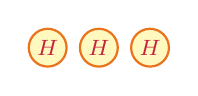
\begin{tikzpicture}[scale=1]
        \foreach \x in {0, 0.65, 1.30} {
          \fill[koreaYellow!80, draw=koreaOrange, thick] (\x,0) circle (0.24) node[font=\bfseries\footnotesize, color=brandCrimson] {$H$};
        }
      \end{tikzpicture}
    \end{minipage}
  \end{minipage}

  \vspace{6pt}
  % PROBLEM 8 (Side-by-side)
  \begin{minipage}{\linewidth}
    \begin{minipage}[c]{0.70\linewidth}
      \exhead{8} ថង់មួយមានឃ្លី $6$ (ខ្មៅ $4$: $ABCD$, ស $2$: $XY$) ។ ចាប់យកម្ដងពីរ ៖
    \end{minipage}\hfill
    \begin{minipage}[c]{0.28\linewidth}
      \centering
      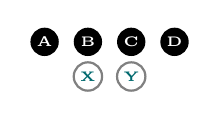
\begin{tikzpicture}[scale=1]
        \foreach \x/\l in {0/A, 0.55/B, 1.1/C, 1.65/D} {
          \fill[black] (\x,0.26) circle (0.18) node[font=\fontsize{4.5}{4.5}\selectfont\bfseries, text=white] {\l};
        }
        \foreach \x/\l in {0.55/X, 1.1/Y} {
          \fill[white, draw=gray, thick] (\x,-0.18) circle (0.18) node[font=\fontsize{4.5}{4.5}\selectfont\bfseries, text=brandNavy] {\l};
        }
      \end{tikzpicture}
    \end{minipage}\\[1.5pt]
    \khlabel{ក} ចាប់បានពណ៌សទាំងពីរ \hfill \khlabel{ខ} ចាប់បានពណ៌ខ្មៅយ៉ាងតិចមួយ
  \end{minipage}
\end{multicols}

\newpage
% =========================================================================
% PAGE 6: SECTION 4 (CONT.): PRACTICE EXERCISES 9 TO 15
% =========================================================================


\begin{multicols}{2}
  \noindent
  % PROBLEM 9
  \exhead{9} គ្រូដាក់សំណួរមេរៀន $6$ ($A, B, C, D, E, F$) ហើយដកស្រង់យក $3$ សំណួរដាក់ឱ្យសិស្សប្រឡង ។ បើសិស្សម្នាក់រៀនបានតែ $4$ សំណួរ ៖\\[1.5pt]
  \khlabel{ក} រកប្រូបាបដែលសិស្សត្រូវ បានពីរសំណួរគត់\\
  \khlabel{ខ} រកប្រូបាបដែលសិស្សត្រូវ បានពីរសំណួរយ៉ាងតិច

  \vspace{6pt}
  % PROBLEM 10
  \exhead{10} ថង់មួយមានឃ្លីស និងខ្មៅសរុប $12$ គ្រាប់ ។ ចាប់ម្ដងមួយ ៖\\[1.5pt]
  \khlabel{ក} រកចំនួនឃ្លីខ្មៅ បើ $P(\text{ខ្មៅ}) = \dfrac{1}{3}$ \\
  \khlabel{ខ} រកប្រូបាបចាប់បានឃ្លីស

  \vspace{6pt}
  % PROBLEM 11 (Side-by-side)
  \begin{minipage}{\linewidth}
    \begin{minipage}[c]{0.70\linewidth}
      \exhead{11} ការិយាល័យមានបុរស $3$ នាក់ និងនារី $2$ នាក់ ។ ជ្រើសរើស $2$ នាក់ដោយចាប់ឆ្នោត ។ រកប្រូបាបដែលជ្រើសបាននារីទាំងពីរនាក់ ។
    \end{minipage}\hfill
    \begin{minipage}[c]{0.28\linewidth}
      \centering
      \begin{tikzpicture}[scale=1]
        \foreach \x in {0, 0.52, 1.04} {
          \fill[brandBlue, rounded corners=2pt] (\x,0) rectangle (\x+0.38,0.32);
          \node[white, font=\fontsize{5.5}{5.5}\selectfont\bfseries] at (\x+0.19,0.16) {ប};
        }
        \foreach \x in {1.60, 2.12} {
          \fill[brandCrimson!80, rounded corners=2pt] (\x,0) rectangle (\x+0.38,0.32);
          \node[white, font=\fontsize{5.5}{5.5}\selectfont\bfseries] at (\x+0.19,0.16) {ន};
        }
      \end{tikzpicture}
    \end{minipage}
  \end{minipage}

  \vspace{6pt}
  % PROBLEM 12 (Side-by-side)
  \begin{minipage}{\linewidth}
    \begin{minipage}[c]{0.68\linewidth}
      \exhead{12} ផ្ទៃថាសខណ្ឌដោយ ៣ ផ្នែកស្មើគ្នា ($A_1, A_2, B$) ។ បង្វិលថាស រួចគប់ព្រួញ ២ ដង ។ រកប្រូបាបគប់បានអក្សរ $A$ ទាំងពីរលើក ។
    \end{minipage}\hfill
    \begin{minipage}[c]{0.30\linewidth}
      \centering
      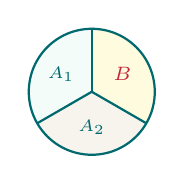
\begin{tikzpicture}[scale=1]
        \coordinate (O) at (0,0);
        \fill[brandTealBg] (O) -- (90:0.80) arc (90:210:0.80) -- cycle;
        \fill[brandLightBlue] (O) -- (210:0.80) arc (210:330:0.80) -- cycle;
        \fill[koreaYellow!40] (O) -- (330:0.80) arc (330:450:0.80) -- cycle;
        \draw[thick, color=brandNavy] (O) circle (0.80);
        \draw[thick, color=brandNavy] (O) -- (90:0.80);
        \draw[thick, color=brandNavy] (O) -- (210:0.80);
        \draw[thick, color=brandNavy] (O) -- (330:0.80);
        \node[font=\fontsize{6.5}{6.5}\selectfont\bfseries, color=brandNavy] at (150:0.45) {$A_1$};
        \node[font=\fontsize{6.5}{6.5}\selectfont\bfseries, color=brandNavy] at (270:0.45) {$A_2$};
        \node[font=\fontsize{7}{7}\selectfont\bfseries, color=brandCrimson] at (30:0.45) {$B$};
      \end{tikzpicture}
    \end{minipage}
  \end{minipage}

  \columnbreak

  % PROBLEM 13 (Side-by-side)
  \begin{minipage}{\linewidth}
    \begin{minipage}[c]{0.70\linewidth}
      \exhead{13} ថង់មួយមានឃ្លីក្រហម $15$ និងឃ្លីខៀវ ។ ចាប់យកឃ្លីមួយដោយចៃដន្យ ដឹងថា $P(\text{ក្រហម}) = \dfrac{3}{5}$ ៖
    \end{minipage}\hfill
    \begin{minipage}[c]{0.28\linewidth}
      \centering
      \begin{tikzpicture}[scale=1]
        \draw[thick, fill=brandTealBg, rounded corners=3pt] (-1.1,-0.28) rectangle (1.1,0.28);
        \node[font=\fontsize{9}{5.5}\selectfont\bfseries, color=brandCrimson] at (-0.45,0) {ក្រ:15};
        \node[font=\fontsize{9}{5.5}\selectfont\bfseries, color=brandBlue] at (0.45,0) {ខ:$x$};
      \end{tikzpicture}
    \end{minipage}\\[1.5pt]
    \khlabel{ក} រកចំនួនឃ្លីពណ៌ខៀវក្នុងថង់\\
    \khlabel{ខ} រកចំនួនឃ្លីក្រហមត្រូវថែម ដើម្បីឱ្យ $P(\text{ក្រហម}) = \dfrac{2}{3}$
  \end{minipage}

  \vspace{6pt}
  % PROBLEM 14 (Side-by-side)
  \begin{minipage}{\linewidth}
    \begin{minipage}[c]{0.70\linewidth}
      \exhead{14} ថ្នាក់រៀនមានស្រី $17$ នាក់ និងប្រុស $23$ នាក់ ។ គ្រូហៅសិស្ស ២ នាក់បន្តបន្ទាប់ដោយចៃដន្យឡើងដោះស្រាយលំហាត់ ៖
    \end{minipage}\hfill
    \begin{minipage}[c]{0.28\linewidth}
      \centering
      \begin{tikzpicture}[scale=1.5]
        \fill[brandCrimson!80, rounded corners=2pt] (0,0) rectangle (0.95,0.30);
        \node[white, font=\fontsize{9}{5.5}\selectfont\bfseries] at (0.475,0.15) {ស្រី:17};
        \fill[brandBlue, rounded corners=2pt] (1.05,0) rectangle (2.0,0.30);
        \node[white, font=\fontsize{9}{5.5}\selectfont\bfseries] at (1.525,0.15) {ប្រុស:23};
      \end{tikzpicture}
    \end{minipage}\\[1.5pt]
    \khlabel{ក} ហៅបានសិស្សស្រីទាំងពីរ \\
     \khlabel{ខ} បានសិស្សប្រុស $\ge 1$\\
    \khlabel{គ} ហៅបានសិស្សទាំងពីរភេទ
  \end{minipage}

  \vspace{6pt}
  % PROBLEM 15 (Side-by-side)
  \begin{minipage}{\linewidth}
    \begin{minipage}[c]{0.70\linewidth}
      \exhead{15} កាក់មួយនិងគ្រាប់ឡុកឡាក់មួយបោះព្រមគ្នា ។ គណនាប្រូបាបបោះកាក់បានខាងរូប និងឡុកឡាក់បានលេខ $6$ ។
    \end{minipage}\hfill
    \begin{minipage}[c]{0.28\linewidth}
      \centering
      \begin{tikzpicture}[scale=1]
        \fill[koreaYellow!80, draw=koreaOrange, thick] (0,0) circle (0.26) node[font=\fontsize{9}{5}\selectfont\bfseries, color=brandCrimson] {រូប};
        \draw[thick, fill=white, rounded corners=2pt] (0.65,-0.25) rectangle (1.15,0.25);
        \fill[brandNavy] (0.78,0.12) circle (0.03);
        \fill[brandNavy] (0.78,0.0) circle (0.03);
        \fill[brandNavy] (0.78,-0.12) circle (0.03);
        \fill[brandNavy] (1.02,0.12) circle (0.03);
        \fill[brandNavy] (1.02,0.0) circle (0.03);
        \fill[brandNavy] (1.02,-0.12) circle (0.03);
      \end{tikzpicture}
    \end{minipage}
  \end{minipage}
\end{multicols}

\end{document}c|c|c|c|c|c|c|c|c|}
        \hline
        \rowcolor{brandNavy!10} \textbf{ថ្ងៃឈប់} & 0 & 1 & 2 & 3 & 4 & 5 & 6 & 7 & 8 \\
        \hline
        \textbf{បុគ្គលិក} & 6 & 1 & 15 & 12 & 24 & 18 & 16 & 10 & 7 \\
        \hline
      \end{tabular}
    \end{center}
    \vspace{-2pt}
    បើគេសម្ភាសន៍បុគ្គលិកម្នាក់ដោយចៃដន្យ រកប្រូបាបដែល ៖\\[1.5pt]
    \khlabel{ក} ឈប់យ៉ាងច្រើន $3$ ថ្ងៃ \hfill \khlabel{ខ} ឈប់យ៉ាងតិច $1$ ថ្ងៃ\\
    \khlabel{គ} ឈប់ចន្លោះ $4$ ទៅ $6$ ថ្ងៃ \hfill \khlabel{ឃ} ឈប់ច្រើនជាង $6$ ថ្ងៃ
  \end{minipage}

  \vspace{4pt}
  % PROBLEM 6 (Side-by-side)
  \begin{minipage}{\linewidth}
    \begin{minipage}[c]{0.60\linewidth}
      \exhead{6} មេអំបៅមួយទំលើផ្កាក្នុងសួន (ស $1$, ក្រហម $2$, ស្វាយ $3$, លឿង $4$) ៖
    \end{minipage}\hfill
    \begin{minipage}[c]{0.38\linewidth}
      \centering
      \begin{tikzpicture}[scale=0.38]
        \draw[thick, fill=koreaOrange!80] (-0.1,0.65) ellipse (0.13 and 0.08);
        \draw[thick, fill=koreaOrange!80] (0.1,0.65) ellipse (0.13 and 0.08);
        \fill[brandNavy] (0,0.65) ellipse (0.025 and 0.1);
        \fill[white, draw=gray, thick] (-1.2,0.06) circle (0.15) node[font=\fontsize{4}{4}\selectfont\bfseries, text=black] {ស1};
        \fill[brandCrimson] (-0.4,0.06) circle (0.15) node[font=\fontsize{4}{4}\selectfont\bfseries, text=white] {ក្រ2};
        \fill[koreaPurple] (0.4,0.06) circle (0.15) node[font=\fontsize{4}{4}\selectfont\bfseries, text=white] {ស្វា3};
        \fill[koreaYellow!90, draw=brandGold, thick] (1.2,0.06) circle (0.15) node[font=\fontsize{4}{4}\selectfont\bfseries, text=brandGold] {លឿង4};
      \end{tikzpicture}
    \end{minipage}\\[1.5pt]
    \khlabel{ក} ពណ៌ស \hfill \khlabel{ខ} ពណ៌ក្រហម \hfill \khlabel{គ} ពណ៌ស្វាយ \hfill \khlabel{ឃ} ពណ៌លឿង
  \end{minipage}

  \vspace{4pt}
  % PROBLEM 7 (Side-by-side)
  \begin{minipage}{\linewidth}
    \begin{minipage}[c]{0.68\linewidth}
      \exhead{7} គេបោះកាក់ម្ដងបី ។ ចូររកប្រូបាបដែលបោះបានមុខ $H$ ទាំងបី ។
    \end{minipage}\hfill
    \begin{minipage}[c]{0.30\linewidth}
      \centering
      
\begin{tikzpicture}[scale=0.36]
        \foreach \x in {0, 0.6, 1.2} {
          \fill[koreaYellow!80, draw=koreaOrange, thick] (\x,0) circle (0.20) node[font=\bfseries\tiny, color=brandCrimson] {$H$};
        }
      \end{tikzpicture}
    \end{minipage}
  \end{minipage}

  \vspace{4pt}
  % PROBLEM 8 (Side-by-side)
  \begin{minipage}{\linewidth}
    \begin{minipage}[c]{0.68\linewidth}
      \exhead{8} ថង់មួយមានឃ្លី $6$ (ខ្មៅ $4$: $ABCD$, ស $2$: $XY$) ។ ចាប់យកម្ដងពីរ ៖
    \end{minipage}\hfill
    \begin{minipage}[c]{0.30\linewidth}
      \centering
      
\begin{tikzpicture}[scale=0.36]
        \foreach \x/\l in {0/A, 0.5/B, 1.0/C, 1.5/D} {
          \fill[black] (\x,0.22) circle (0.15) node[font=\fontsize{4}{4}\selectfont\bfseries, text=white] {\l};
        }
        \foreach \x/\l in {0.5/X, 1.0/Y} {
          \fill[white, draw=gray, thick] (\x,-0.12) circle (0.15) node[font=\fontsize{4}{4}\selectfont\bfseries, text=brandNavy] {\l};
        }
      \end{tikzpicture}
    \end{minipage}\\[1.5pt]
    \khlabel{ក} ចាប់បានពណ៌សទាំងពីរ \hfill \khlabel{ខ} ចាប់បានពណ៌ខ្មៅយ៉ាងតិចមួយ
  \end{minipage}
\end{multicols}

\newpage
% =========================================================================
% PAGE 6: SECTION 4 (CONT.): PRACTICE EXERCISES 9 TO 15
% =========================================================================
\khsection{៤}{លំហាត់អនុវត្តន៍បន្ថែម (ត)}

\begin{multicols}{2}
  \noindent
  % PROBLEM 9
  \exhead{9} គ្រូដាក់សំណួរមេរៀន $6$ ($A, B, C, D, E, F$) ហើយដកស្រង់យក $3$ សំណួរដាក់ឱ្យសិស្សប្រឡង ។ បើសិស្សម្នាក់រៀនបានតែ $4$ សំណួរ ៖\\[1.5pt]
  \khlabel{ក} រកប្រូបាបដែលសិស្សត្រូវ បានពីរសំណួរគត់\\
  \khlabel{ខ} រកប្រូបាបដែលសិស្សត្រូវ បានពីរសំណួរយ៉ាងតិច

  \vspace{3pt}
  % PROBLEM 10
  \exhead{10} ថង់មួយមានឃ្លីស និងខ្មៅសរុប $12$ គ្រាប់ ។ ចាប់ម្ដងមួយ ៖\\[1.5pt]
  \khlabel{ក} រកចំនួនឃ្លីខ្មៅ បើ $P(\text{ខ្មៅ}) = \dfrac{1}{3}$ \hfill \khlabel{ខ} រកប្រូបាបចាប់បានឃ្លីស

  \vspace{3pt}
  % PROBLEM 11 (Side-by-side)
  \begin{minipage}[c]{0.64\linewidth}
    \exhead{11} ការិយាល័យមានបុរស $3$ នាក់ និងនារី $2$ នាក់ ។ ជ្រើសរើស $2$ នាក់ដោយចាប់ឆ្នោត ។ រកប្រូបាបដែលជ្រើសបាននារីទាំងពីរនាក់ ។
  \end{minipage}\hfill
  \begin{minipage}[c]{0.34\linewidth}
    \centering
    \begin{tikzpicture}[scale=0.35]
      \foreach \x in {0, 0.48, 0.96} {
        \fill[brandBlue, rounded corners=1.5pt] (\x,0) rectangle (\x+0.32,0.26);
        \node[white, font=\fontsize{4.5}{4.5}\selectfont\bfseries] at (\x+0.16,0.13) {ប};
      }
      \foreach \x in {1.55, 2.03} {
        \fill[brandCrimson!80, rounded corners=1.5pt] (\x,0) rectangle (\x+0.32,0.26);
        \node[white, font=\fontsize{4.5}{4.5}\selectfont\bfseries] at (\x+0.16,0.13) {ន};
      }
    \end{tikzpicture}
  \end{minipage}

  \vspace{3pt}
  % PROBLEM 12 (Side-by-side)
  \begin{minipage}[c]{0.66\linewidth}
    \exhead{12} ផ្ទៃថាសខណ្ឌដោយ ៣ ផ្នែកស្មើគ្នា ($A_1, A_2, B$) ។ បង្វិលថាស រួចគប់ព្រួញ ២ ដង ។ រកប្រូបាបគប់បានអក្សរ $A$ ទាំងពីរលើក ។
  \end{minipage}\hfill
  \begin{minipage}[c]{0.32\linewidth}
    \centering
    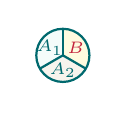
\begin{tikzpicture}[scale=0.45]
      \coordinate (O) at (0,0);
      \fill[brandTealBg] (O) -- (90:0.75) arc (90:210:0.75) -- cycle;
      \fill[brandLightBlue] (O) -- (210:0.75) arc (210:330:0.75) -- cycle;
      \fill[koreaYellow!40] (O) -- (330:0.75) arc (330:450:0.75) -- cycle;
      \draw[thick, color=brandNavy] (O) circle (0.75);
      \draw[thick, color=brandNavy] (O) -- (90:0.75);
      \draw[thick, color=brandNavy] (O) -- (210:0.75);
      \draw[thick, color=brandNavy] (O) -- (330:0.75);
      \node[font=\fontsize{6}{6}\selectfont\bfseries, color=brandNavy] at (150:0.42) {$A_1$};
      \node[font=\fontsize{6}{6}\selectfont\bfseries, color=brandNavy] at (270:0.42) {$A_2$};
      \node[font=\fontsize{6.5}{6.5}\selectfont\bfseries, color=brandCrimson] at (30:0.42) {$B$};
    \end{tikzpicture}
  \end{minipage}

  \columnbreak

  % PROBLEM 13 (Side-by-side)
  \begin{minipage}[c]{0.64\linewidth}
    \exhead{13} ថង់មួយមានឃ្លីក្រហម $15$ និងឃ្លីខៀវ ។ ចាប់យកឃ្លីមួយដោយចៃដន្យ ដឹងថា $P(\text{ក្រហម}) = \dfrac{3}{5}$ ៖
  \end{minipage}\hfill
  \begin{minipage}[c]{0.34\linewidth}
    \centering
    \begin{tikzpicture}[scale=0.36]
      \draw[thick, fill=brandTealBg, rounded corners=2pt] (-1.1,-0.2) rectangle (1.1,0.2);
      \node[font=\fontsize{4.5}{4.5}\selectfont\bfseries, color=brandCrimson] at (-0.4,0) {ក្រ:15};
      \node[font=\fontsize{4.5}{4.5}\selectfont\bfseries, color=brandBlue] at (0.4,0) {ខ:$x$};
    \end{tikzpicture}
  \end{minipage}\\[1.5pt]
  \khlabel{ក} រកចំនួនឃ្លីពណ៌ខៀវក្នុងថង់\\
  \khlabel{ខ} រកចំនួនឃ្លីក្រហមត្រូវថែម ដើម្បីឱ្យ $P(\text{ក្រហម}) = \dfrac{2}{3}$

  \vspace{3pt}
  % PROBLEM 14 (Side-by-side)
  \begin{minipage}[c]{0.64\linewidth}
    \exhead{14} ថ្នាក់រៀនមានស្រី $17$ នាក់ និងប្រុស $23$ នាក់ ។ គ្រូហៅសិស្ស ២ នាក់បន្តបន្ទាប់ដោយចៃដន្យឡើងដោះស្រាយលំហាត់ ៖
  \end{minipage}\hfill
  \begin{minipage}[c]{0.34\linewidth}
    \centering
    \begin{tikzpicture}[scale=0.36]
      \fill[brandCrimson!80, rounded corners=1.5pt] (0,0) rectangle (0.85,0.24);
      \node[white, font=\fontsize{4.5}{4.5}\selectfont\bfseries] at (0.425,0.12) {ស្រី:17};
      \fill[brandBlue, rounded corners=1.5pt] (0.95,0) rectangle (1.8,0.24);
      \node[white, font=\fontsize{4.5}{4.5}\selectfont\bfseries] at (1.375,0.12) {ប្រុស:23};
    \end{tikzpicture}
  \end{minipage}\\[1.5pt]
  \khlabel{ក} ហៅបានសិស្សស្រីទាំងពីរ \hfill \khlabel{ខ} បានសិស្សប្រុស $\ge 1$\\
  \khlabel{គ} ហៅបានសិស្សទាំងពីរភេទ

  \vspace{3pt}
  % PROBLEM 15 (Side-by-side)
  \begin{minipage}[c]{0.68\linewidth}
    \exhead{15} កាក់មួយនិងគ្រាប់ឡុកឡាក់មួយបោះព្រមគ្នា ។ គណនាប្រូបាបបោះកាក់បានខាងរូប និងឡុកឡាក់បានលេខ $6$ ។
  \end{minipage}\hfill
  \begin{minipage}[c]{0.30\linewidth}
    \centering
    \begin{tikzpicture}[scale=0.35]
      \fill[koreaYellow!80, draw=koreaOrange, thick] (0,0) circle (0.20) node[font=\fontsize{3.5}{3.5}\selectfont\bfseries, color=brandCrimson] {រូប};
      \draw[thick, fill=white, rounded corners=1.5pt] (0.55,-0.20) rectangle (0.95,0.20);
      \fill[brandNavy] (0.65,0.10) circle (0.025);
      \fill[brandNavy] (0.65,0.0) circle (0.025);
      \fill[brandNavy] (0.65,-0.10) circle (0.025);
      \fill[brandNavy] (0.85,0.10) circle (0.025);
      \fill[brandNavy] (0.85,0.0) circle (0.025);
      \fill[brandNavy] (0.85,-0.10) circle (0.025);
    \end{tikzpicture}
  \end{minipage}
\end{multicols}

\end{document}
